
\section{Polymorphism}
\label{sec:polymorphyism}

Polymorphism is the ability of an entity to show diferent shapes or
forms. In biology, polymorphic animals can exist isa variety of
different forms, e.g.~male and female animals, or different blood
types. In materials science, polymorphic material can exist in a
variety of different crystaline configurations (e.g.~calcite and
aragonite). 

In computer science, polymorphism appears at many levels. In
Programming in Java, we interested in two types of polymorphism:
polymorphic classes and polymorphic methods. The former is usually
referred to as \emph{generic types}, while the latter is usually
called \emph{method overloading}. 

\section{Generic types}
\label{sec:generic-types}

...


\section{Method overloading}
\label{sec:method-overloading}

...

\section{Introduction to upcasting}
\label{sec:upcasting}

There is a third type of
polymorphism in Java that is simpler but very important. We have
already seen how it works, although we have not used its proper name
until now.
%We are already familiar with \emph{upcasting}, although we have not
%called it like that. 
We have been using it every time we have declared
a variable by using an interface: 

\begin{verbatim}
    List patientList;
    patientList = new ArrayPatientList();
\end{verbatim}

We know that it is good practice to work with interface names for our
data types, rather than to use the class names directly. The interface
allows the programmer to abstract from all the implementation details
of the class and work with just its public behaviour, i.e.~the methods
defined on the interface. This is upcasting, and it is similar to the
casting of simple types we have already seen; you just need to know
that, by convention, interfaces are imagined to be ``up'' and specific
classes are imagined to be ``down'', so casting from class to
interface is up-casting. (The origin in computer science is almost
always up: the root of a tree, the interface of a class, etc). 

\begin{figure}[hbtp]
  \centering
  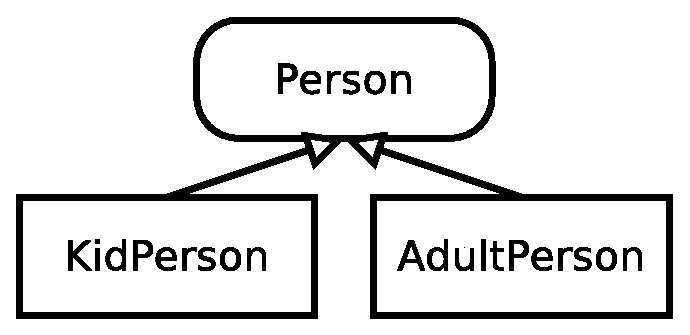
\includegraphics[height=3cm]{gfx/class_diagram-person}
  \caption{Interface Person is implemented by classes KidPerson and
    AdultPerson. By convention, the interface is represented ``up'' and
    the classes are represented ``down''.} 
  \label{fig:updown}
\end{figure}

We will see more about upcasting (and downcasting) in the following
sections. 



%%% Local Variables:
%%% mode: latex
%%% TeX-master: "main"
%%% End:
